%%% LaTeX Template: Two column article
%%%
%%% Source: http://www.howtotex.com/
%%% Feel free to distribute this template, but please keep to referal to http://www.howtotex.com/ here.
%%% Date: February 2011

%%% Preamble
\documentclass[	DIV=calc,%
							paper=a4,%
							fontsize=12pt,%
							onecolumn]{scrartcl}	 					% KOMA-article class
							
\usepackage{url}

\usepackage{lipsum}													% Package to create dummy text
\usepackage[brazil]{babel}										% English language/hyphenation
\usepackage[protrusion=true,expansion=true]{microtype}				% Better typography
\usepackage{amsmath,amsfonts,amsthm}					% Math packages
\usepackage[pdftex]{graphicx}									% Enable pdflatex
\usepackage[svgnames]{xcolor}									% Enabling colors by their 'svgnames'
\usepackage[hang, small,labelfont=bf,up,textfont=it,up]{caption}	% Custom captions under/above floats
\usepackage{epstopdf}												% Converts .eps to .pdf
\usepackage{subfig}													% Subfigures
\usepackage{booktabs}												% Nicer tables
\usepackage{fix-cm}													% Custom fontsizes
\usepackage[utf8]{inputenc}
\usepackage[top=2.5cm, bottom=2.5cm, left=2.5cm, right=2.5cm]{geometry}
\usepackage[ddmmyyyy]{datetime}
\addto\captionsenglish{%
	\renewcommand\tablename{Tabela}
	\renewcommand\figurename{Figura}
} 
 

\usepackage{float}
 
%%% Custom sectioning (sectsty package)
\usepackage{sectsty}													% Custom sectioning (see below)
\allsectionsfont{%															% Change font of al section commands
	\usefont{OT1}{phv}{b}{n}%										% bch-b-n: CharterBT-Bold font
	}

\sectionfont{%																% Change font of \section command
	\usefont{OT1}{phv}{b}{n}%										% bch-b-n: CharterBT-Bold font
	}



%%% Headers and footers
\usepackage{fancyhdr}												% Needed to define custom headers/footers
	\pagestyle{fancy}														% Enabling the custom headers/footers
\usepackage{lastpage}	

% Header (empty)
\lhead{}
\chead{}
\rhead{}
% Footer (you may change this to your own needs)

%% ====================================
%% ====================================
%% mude o rodape  do projeto
%% ====================================
%% ====================================

\lfoot{\footnotesize \texttt{Cabeamento estruturado} \textbullet ~Centro Universitário Internacional - Uninter}


\cfoot{}
\rfoot{\footnotesize página \thepage\ de \pageref{LastPage}}	% "Page 1 of 2"
\renewcommand{\headrulewidth}{0.0pt}
\renewcommand{\footrulewidth}{0.4pt}



%%% Creating an initial of the very first character of the content
\usepackage{lettrine}
\newcommand{\initial}[1]{%
     \lettrine[lines=3,lhang=0.3,nindent=0em]{
     				\color{DarkGoldenrod}
     				{\textsf{#1}}}{}}



%%% Title, author and date metadata
\usepackage{titling}															% For custom titles

\newcommand{\HorRule}{\color{DarkGoldenrod}%			% Creating a horizontal rule
									  	\rule{\linewidth}{1pt}%
										}

\pretitle{\vspace{-30pt} \begin{flushleft} \HorRule 
				\fontsize{40}{50} \usefont{OT1}{phv}{b}{n} \color{DarkRed} \selectfont 
				}

%% ====================================
%% ====================================
%% mude o titulo  do projeto
%% ====================================
%% ====================================

\title{Cabeamento Estruturado do Centro Universitário Internacional - Uninter}					% Title of your article goes here

%% ====================================



\posttitle{\par\end{flushleft}\vskip 0.5em}

\preauthor{\begin{flushleft}
					\large \lineskip 0.5em \usefont{OT1}{phv}{b}{sl} \color{DarkRed}}
\author{Eliseu Philippe Cavalaro Santos Machado}  	% Author name goes here


\postauthor{\footnotesize \usefont{OT1}{phv}{m}{sl} \color{Black} 
					\\Universidade Tecnológica Federal do Paraná - Câmpus Cornélio Procópio 								% Institution of author
					\par\end{flushleft}\HorRule}

\date{}
% No date




%%% Begin document
\begin{document}
\maketitle
\thispagestyle{fancy} 	
\thispagestyle{empty}		% Enabling the custom headers/footers for the first page 
% The first character should be within \initial{}




%% ====================================
%% ====================================
%% mude o resumo  do projeto
%% ====================================
%% ====================================
\initial{E}\textbf{ste projeto tem como objetivo de apresentar de forma fictícia o cabeamento estruturado para um Polo de uma Universidade à distância, pois será preciso elaborar do zero toda a estrutura de cabos.
	O projeto abrange levantamento da planta física, equipamentos passivos na rede, levantamento da quantidade e custo, certificação, orçamento e riscos que devem ser levados em conta.}

%% ====================================
\begin{figure}
	\centering
	
\includegraphics{utfpr}
\end{figure}

\vspace{3cm}
\centerline{\textit{\textbf{\today}}}

\clearpage
    \renewcommand*\listfigurename{Lista de figuras}
\listoffigures

\renewcommand*\listtablename{Lista de tabelas}
\listoftables




\clearpage
\renewcommand{\contentsname}{Sumário}
\tableofcontents
\clearpage

%% ====================================
%% ====================================
%% Inicio do texto
%% ====================================
%% ====================================
\section{Introdução}
Este projeto tem o intuito de planejar a elaboração de um cabeamento estruturado em uma universidade à distância, para um novo prédio, no qual, não há infraestrutura de redes alguma. 
Segundo Fey (2014) \cite{ref1}, acerca do cabeamento estruturado, no qual surgiu da necessidade de se padronizar toda e qualquer instalação de telecomunicação em prédios comerciais, devido ao surgimento das redes locais no final da década de 1980. Essas normas tiveram papel fundamental, uma vez que recomendavam aspectos técnicos visando padronizar os projetos, instalações e testes de certificação.
O PAP (Polo de Apoio Presencial) fica situado na cidade de Itararé-SP e faz parte do Centro Universitário Internacional – Uninter, que conta com 9 (nove) colaboradores.
A organização tem 22 (vinte e dois) computadores de mesa, 3 (três) roteadores wireless, 5 (cinco) switches, 3 (três) impressoras na rede.
O polo necessita de uma sala para o laboratório de informática, onde os alunos possam estar realizando avaliações, trabalhos e atividades, com a necessidade de softwares específicos para realização das mesmas. Além de outras salas, como tutorias, coordenação, secretaria e biblioteca, todas com acesso de forma cabeada à rede, além da conexão sem fio para os alunos.
Portanto, o objetivo deste projeto é apenas estabelecer a estruturação dos cabos da camada física, ou seja, a disponibilização dos pontos de redes. A configuração de switches, roteadores e demais ativos, não faz parte do escopo deste projeto.

\subsection{Benefícios}
\begin{itemize}
	\item Redução de custos a longo prazo;
	\item Redução na manutenção da camada física;
	\item Padronização da estrutura;
	\item Possibilidade de expansão futura;
	\item Flexibilidade e agilidade nos processos de mudança;
	\item Redução de ativos na rede.
\end{itemize}

\subsection{Organizações Envolvidas}
\begin{table}[H]
	\centering
	\caption{Organizações Envolvidas}
	\label{my-label}
	\begin{tabular}{|l|l|}
		\hline
		João da Silva ME & Responsável pela estrutura de cabos e eltrodutos na rede elétrica \\ \hline
		José Antônio ME  & Responsável pela estrutura de cabos de dados e eletrodutos        \\ \hline
	\end{tabular}
\end{table}



\section{Estado atual}
Será implementado um novo cabeamento.

\section{Requisitos}
\begin{enumerate}
	\item Melhorar o fluxo de informações e desempenho no segmento de rede;
	\item Padronizar as instalações de infraestrutura;
	\item Organizar o cabeamento e identificá-los;
	\item Possibilitar futura expansão.	
\end{enumerate}

\section{Usuários e Aplicativos}
No total são 9 (nove) usuários fixos, ou seja, os colaboradores. Porém, os alunos também utilizam a rede, o que varia, podendo chegar a 200 (duzentas) conexões simultâneas. Como se trata de uma faculdade à distância existe a possibilidade de expansão tanto para funcionários quanto principalmente em relação aos alunos.
 

\subsection{Usuários}
Como são 9 (nove) colaboradores, esses são sempre os que utilizam a rede a todo momento, mas existe a possibilidade desse número aumentar devido a demanda de alunos que também utilizam a rede em épocas que variam.

\subsection{Aplicativos}
Apenas e-mails, softwares que rodam localmente, aplicativos de provas, não gerando um grande fluxo na rede.


\section{Estrutura predial existente}
\begin{figure}[H]
	\centering
	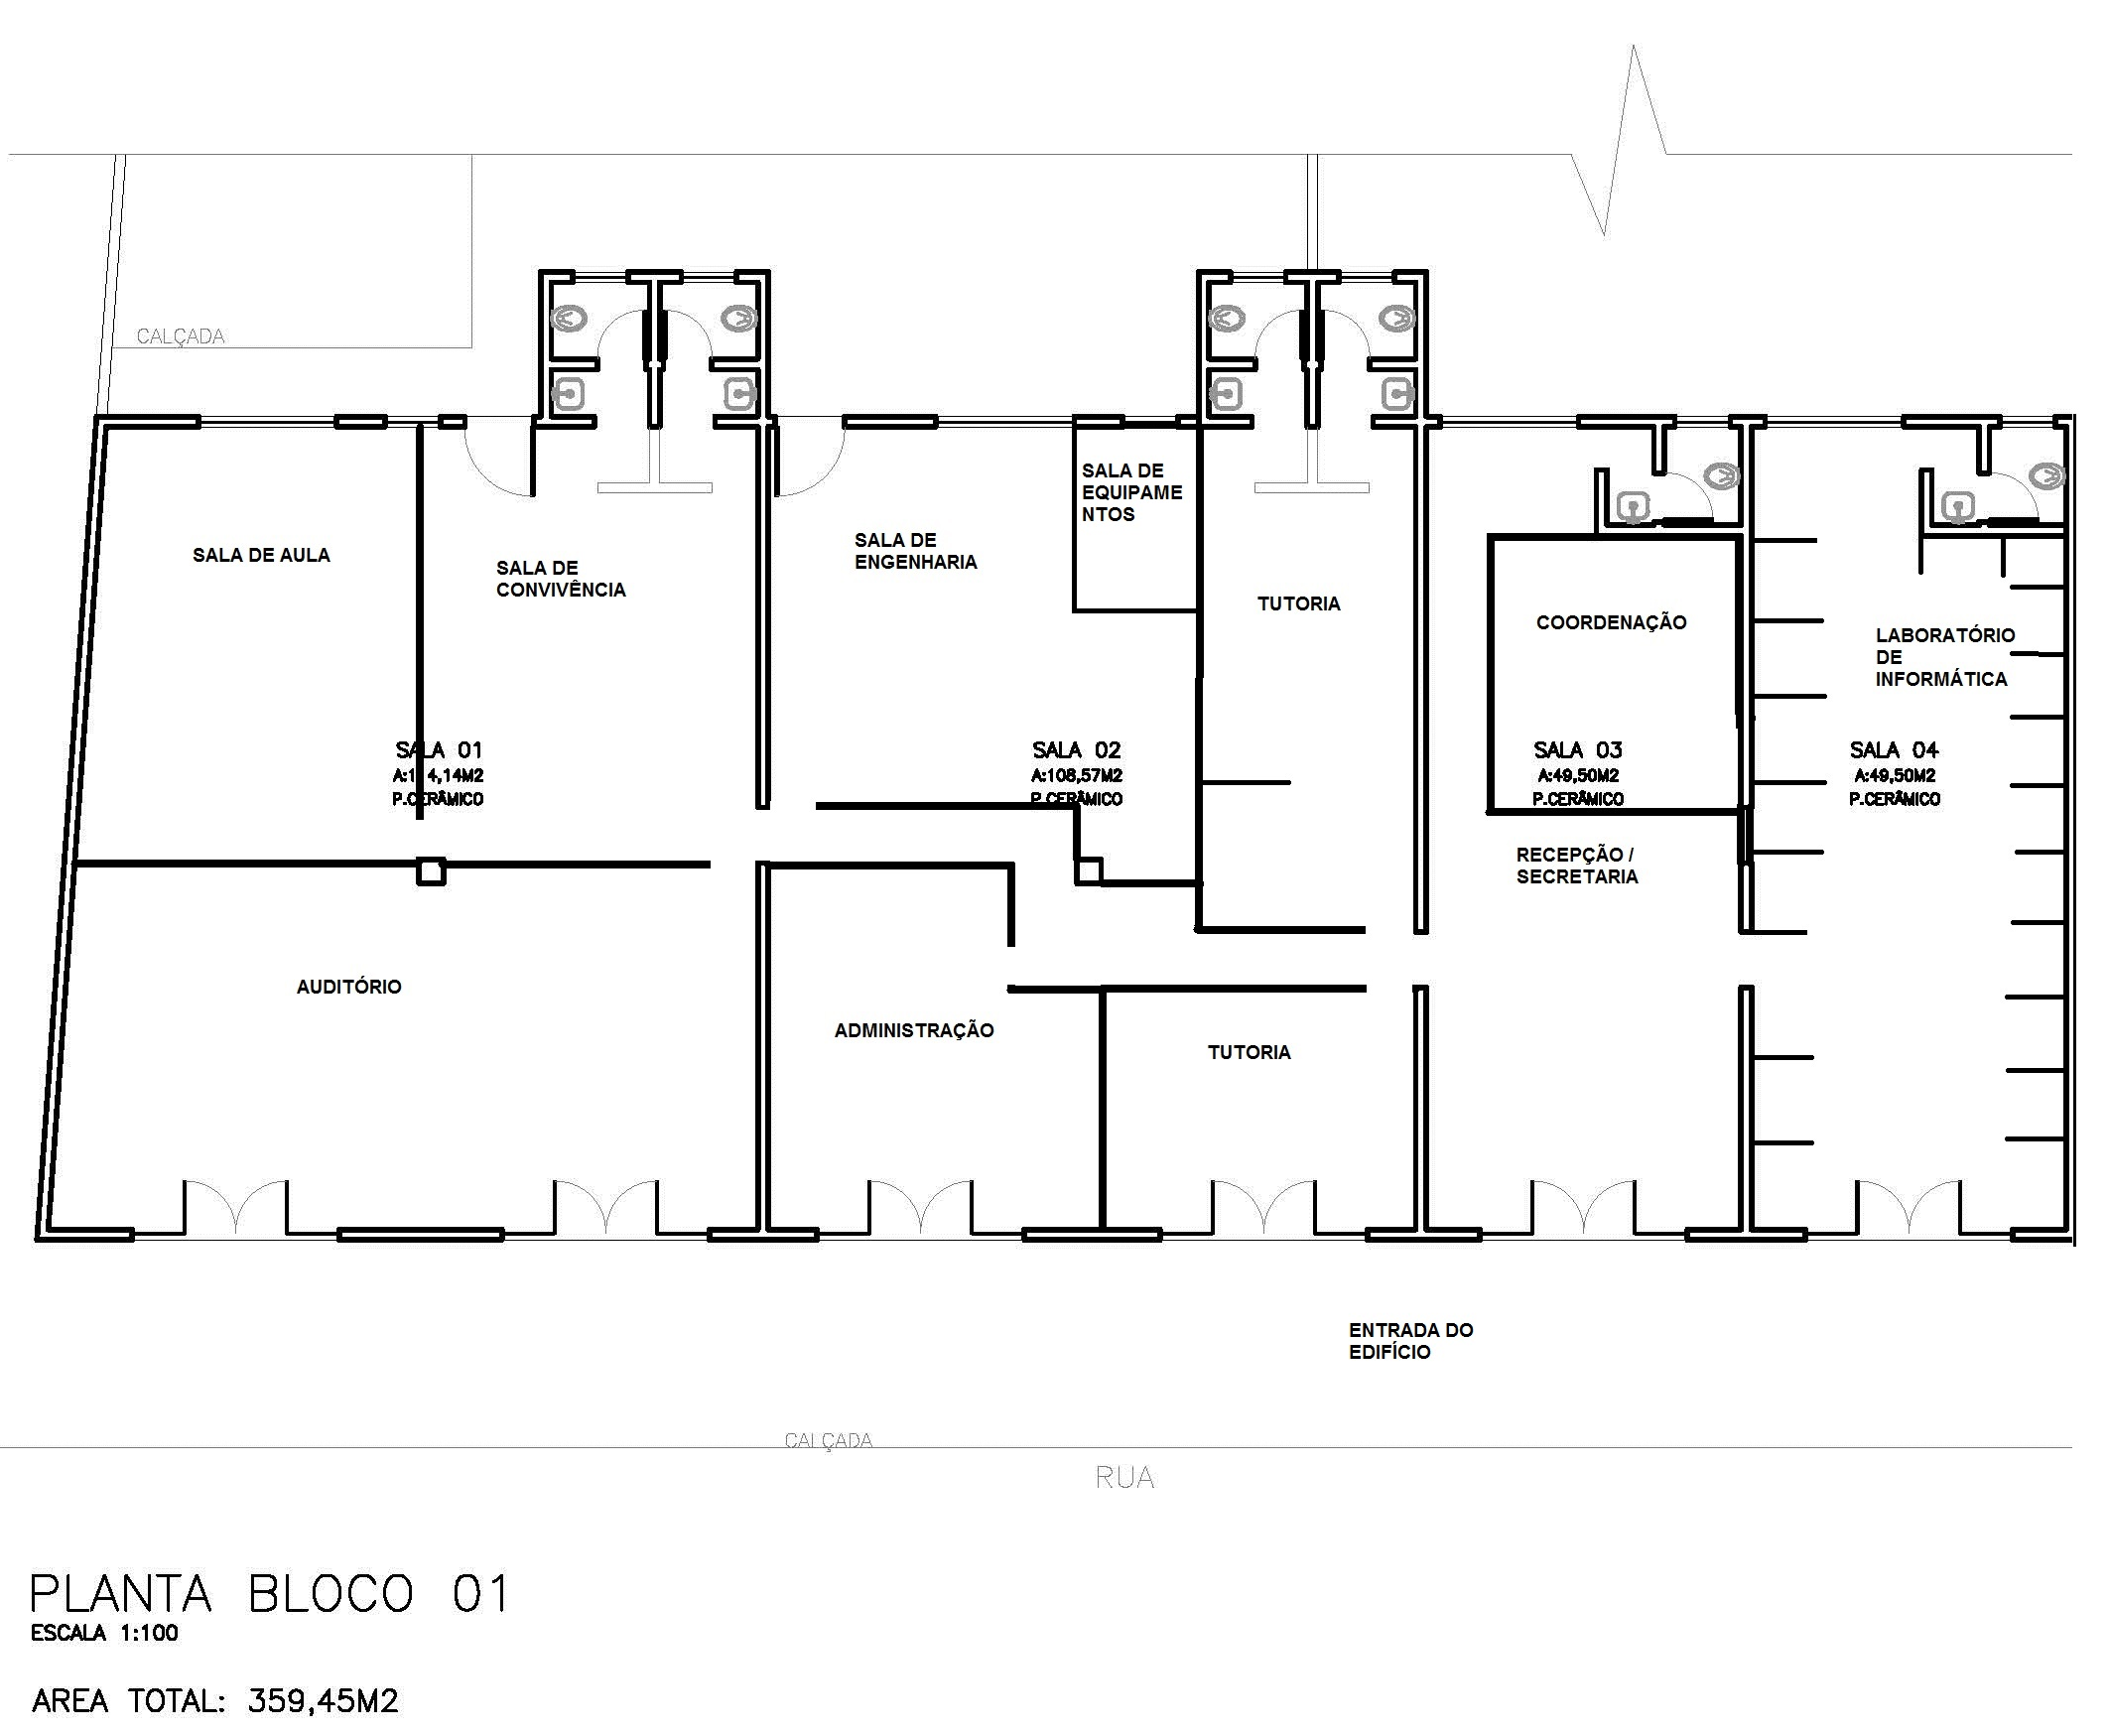
\includegraphics[scale=0.25]{planta1}
	\caption{Estrutura do prédio}
	\label{planta1}
\end{figure}

\section{Planta Lógica - Elementos estruturados}

\subsection{Estado atual}
Não há.

\subsection{Topologia}
A topologia utilizada será a estrela, como o prédio se encontra no térreo com divisórias nas salas, haverá apenas uma sala de equipamentos com um rack, no qual fará toda a distribuição do cabeamento. Nele, serão instalados todos os passivos e ativos.
Existem 6 (seis) características no cabeamento estruturado:
\begin{itemize}
	\item Entrada do Edifício: as instalações de entrada fornecem a interface entre o cabeamento interno com o externo (provedor de internet);
	\item Área de Trabalho: compreende a área destinada ao trabalho dos usuários, como também, terminais de dados, telefones, tomadas de rede, etc.;
	\item Cabeamento Horizontal: é a interligação da sala de equipamentos e / ou telecomunicações com a área de trabalho, finalizando nas tomadas de rede;
	\item Cabeamento Vertical: é a interligação entre a sala de equipamentos com as salas de telecomunicações (utilizado em prédios com mais de 1 (um) andar);
	\item Sala de Equipamentos: possui os equipamentos com maior complexidade, como, servidores, CFTV, centrais de telefone, roteadores;
	\item Sala de Telecomunicações: tem como função distribuir o cabeamento horizontal para a área de trabalho do andar e receber o cabeamento vertical do backbone.
\end{itemize}

\begin{figure}[H]
	\centering
	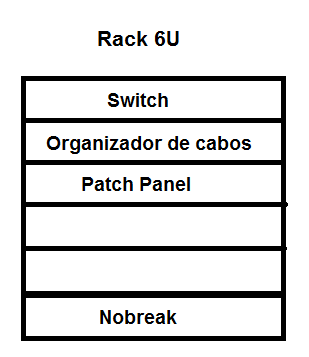
\includegraphics[scale=0.5]{rack}
	\caption{Protótipo de organização do rack}
	\label{rack}
\end{figure}

\subsection{Encaminhamento}
A instalação será feita externamente, através de eletro dutos, no qual passará todo o cabeamento até os pontos de rede.

\subsection{Memorial descritivo}

\begin{table}[H]
	\centering
	\caption{Memorial Descritivo}
	\label{my-label}
	\begin{tabular}{|c|c|c|c|}
		\hline
		\textbf{NOME}                                                                                 & \textbf{TIPO}            & \textbf{FABRICANTE} & \textbf{QUANTIDADE} \\ \hline
		CABO DE REDE                                                                         & CAT5e           & FURUKAWA   & 2000m      \\ \hline
		CONECTOR MACHO                                                                       & RJ45            & FURUKAWA   & 100        \\ \hline
		CONECTOR FÊMEA                                                                       & CAT5e KEYSTONE  & FURUKAWA   & 50         \\ \hline
		ESPELHO                                                                              & 4X2             & -          & 25         \\ \hline
		PATCH PANEL                                                                          & 24 PORTAS CAT5e & FURUKAWA   & 1          \\ \hline
		ELETRODUTO                                                                           & PVC             & -          & -          \\ \hline
		\begin{tabular}[c]{@{}c@{}}ETIQUETAS DE \\ \\ IDENTIFICAÇÃO\\ DOS CABOS\end{tabular} & -               & -          & 200        \\ \hline
	\end{tabular}
\end{table}

\subsection{Identificação dos cabos}
Com base nas Norma EIA/TIA - 606, que rege sobre a identificação, organização e administração do cabeamento, será feito da seguinte forma \cite{ref1}:

\begin{table}[H]
	\centering
	\caption{Formato de Identificação do cabeamento estruturado, adaptado \cite{ref1}}
	\label{my-label}
	\begin{tabular}{|c|c|c|}
		\hline
		ELEMENTO                                                            & IDENTIFICAÇÃO / SIGNIFICADO                                                                                                    & EXEMPLO                                                                                                                                                                                               \\ \hline
		\begin{tabular}[c]{@{}c@{}}TOMADA DE\\ TELECOMUNICAÇÃO\end{tabular} & \begin{tabular}[c]{@{}c@{}}TO XX xxx\\ XX - Andar\\ xxx - sequencial\end{tabular}                                              & \begin{tabular}[c]{@{}c@{}}TO 02 026\\ \\ Tomada 026 do 2º andar\end{tabular}                                                                                                                         \\ \hline
		PONTAS DOS CABOS UTP                                                & \begin{tabular}[c]{@{}c@{}}CWY XX XXX\\ W: P - Primário, I - Interligação\\ Y: U- UTP, S - STP, Fo - Fibra Óptica\end{tabular} & \begin{tabular}[c]{@{}c@{}}CSU 03 008\\ Cabo 008 do tipo UTP, \\ \\ Secundário e do 3º andar\end{tabular}                                                                                             \\ \hline
		TRECHOS DE CABOS UTP                                                & \begin{tabular}[c]{@{}c@{}}NNx CWY nnP\\ XX xxx a xxx\\ NN: Quantidade de cabos\\ nn: quantidade de pares\end{tabular}         & \begin{tabular}[c]{@{}c@{}}03 x CPU 02P\\ 02 005 a008\\ 3 cabos UTP de 2 pares,\\ primários e que se destinam\\ ao segundo pavimento. Os \\ \\ cabos são de sequência \\ \\ 005 até 008.\end{tabular} \\ \hline
	\end{tabular}
\end{table}

\section{Implantação}
\begin{figure}[H]
	\centering
	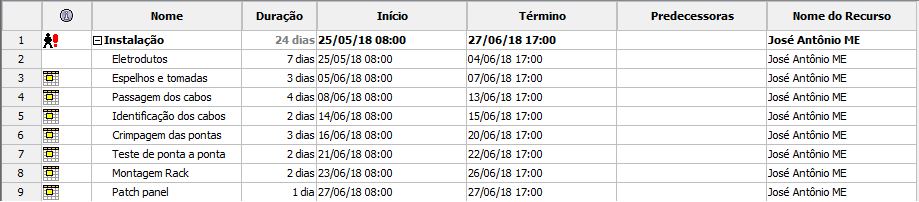
\includegraphics[scale=0.65]{cronograma}
	\caption{Cronograma das tarefas realizadas}
	\label{cronograma}
\end{figure}

\section{Plano de certificação}
A certificação é de suma importância, uma vez que previne problemas futuros com o uso da rede, verificando o cumprimento das normas e regulamentação, assim, permite encontrar qualquer anomalia e aponta os problemas causados pela má qualidade dos passivos, afirma Fey (2014) \cite{ref1}.

A certificação será realizada logo que a camada física for implementada, antes mesmo do uso real da rede, a fim de evitar problemas durante o utilização da mesma. Para a certificação usa-se um equipamento específico, no qual, gera um relatório que aponta se a rede está adequada ou não. A rede toda será certificada.

Segundo Samuel \cite{ref2}, Fey (2014) \cite{ref1} e Pena \cite{ref3}, as etapas da certificação são:
\begin{itemize}
	\item Wiremap: verifica a paridade dos cabos, e se não há nenhum fio invertido. Em caso de falha, provavelmente há algum cabo injetado incorretamente;
	\item Wire Lenght: verifica o comprimento dos cabos;
	\item Teste de Resistência: mede a resistência de circuito de cada par de fio;
	\item NEXT (Near-End Cross Talk): diz respeito a interferência entre pares de fios na mesma extremidade;
	\item FEXT (Far-End Cross Talk): é o contrário do NEXT, verifica a interferência entre pares de fios em extremidades opostas de um mesmo cabo;
	\item Atenuação: verifica a perda de potência do sinal transmitido, quanto maior a frequência do sinal, pior;
	\item Return Loss: mede a proporção da potência do sinal transmitido e refletido. Cabos bons têm poucos sinais refletidos;
	\item Impedância: mais um teste que verifica danos físicos nos cabos, se foi esmagado ou muito esticado;
	\item Delay: é o período de tempo em que o sinal leva para chegar de uma extremidade a outra;
	\item Skew: relata a diferença entre o maior e o menor tempo;
	\item Capacitância: mede a capacidade mútua entre os dois condutores de cada par e verifica se a instalação não afetou a capacidade do cabo de transmitir o sinal.

\end{itemize}



\section{Plano de manutenção}

As revisões serão feitas a cada 3 (três) meses, com o intuito de evitar problemas maiores. Caso haja a necessidade de adicionar um novo ponto, deverá ser feita uma certificação neste ponto em questão seguindo os passos do item acima. 

\subsection{Plano de expansão}
A rede poderá ser expandida na medida em que os pontos serão instalados, uma vez que cada espelho terá 2 (dois) pontos.

\section{Risco}
É preciso planejar certos riscos na implementação do cabeamento estruturado, como:
\begin{enumerate}
	\item Má instalação dos cabos de rede UTP, evitar esticar demais, esmagar;
	\item Má crimpagem dos conectores de patch-cord;
	\item Manuseio incorreto do punch-down ao adicionar um ponto;
	\item Passivos de má qualidade.
	
\end{enumerate}
A equipe responsável pela instalação e manuseio deverá ser totalmente treinada e capacitada, a fim de evitar problemas maiores.

\section{Orçamento}
\begin{table}[H]
	\centering
	\caption{Orçamento dos materiais}
	\label{my-label}
	\begin{tabular}{|c|c|c|c|c|}
		\hline
		\textbf{NOME}                                                                             & \textbf{TIPO}                                                            & \textbf{FABRICANTE} & \textbf{QUANTIDADE} & \textbf{PREÇO}       \\ \hline
		Cabo de rede                                                                     & Cat5e                                                           & Furukawa   & 2.000 m    & R\$ 2.373,00 \\ \hline
		Conector Macho                                                                   & RJ45                                                            & Furukawa   & 100        & R\$ 85,00    \\ \hline
		Espelho                                                                          & 4x2                                                             & -          & 25         & R\$ 170,00   \\ \hline
		Conector Fêmea                                                                   & \begin{tabular}[c]{@{}c@{}}RJ45 KeyStone\\   Cat5e\end{tabular} & Furukawa   & 50         & R\$ 325,00   \\ \hline
		\begin{tabular}[c]{@{}c@{}}Patch Panel 24\\   portas\end{tabular}                & Cat5e                                                           & Furukawa   & 1          & R\$ 145,00   \\ \hline
		Eletroduto                                                                       & PVC                                                             & -          & 3.000m     & R\$ 2.580,00 \\ \hline
		\begin{tabular}[c]{@{}c@{}}Etiquetas de\\   Identificação dos cabos\end{tabular} & -                                                               & -          & 200        & R\$ 280,00   \\ \hline
	\end{tabular}
\end{table}

Total: R\$ 5.958,00.

\section{Recomendações}
Deve-se atentar ao manuseio correto ao plugar e desplugar patch-cords da parede e do equipamento. Em caso de problemas de conectividade, deverá ser relatado ao departamento de TI ou responsável.

\section{Referências bibliográficas}
\renewcommand\refname{} %%Referências bibliográficas}  
\bibliographystyle{ieeetr}
\bibliography{referencias}  


\end{document}